\documentclass[a4paper, 14pt]{extarticle}
\usepackage{../generalPreamble}
\usepackage{../conspectFormat}
\usepackage{../nonFancyTOC}
\usepackage{../russianLocale}

\lhead{}

\title{Экзаменационные вопросы по ЦОС}
\author{Корытов Павел, 6304 \\ Лектор: Дмитрий Клионский\\ СПбГЭТУ \enquote{ЛЭТИ}}
\date{\today}
\begin{document}
{\small
\maketitle
}

\setcounter{secnumdepth}{4}
\setcounter{tocdepth}{1}
\tableofcontents{}
\section{Обобщенная схема ЦОС}
\begin{figure}[h]
    \centering
    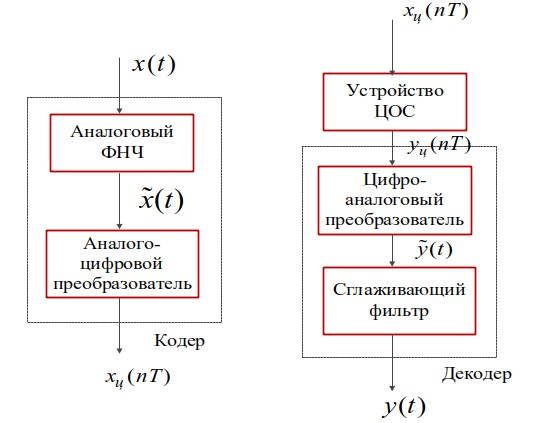
\includegraphics[width=0.4\textwidth]{img/S001.jpg}
\end{figure}
Исходная информация в обобщенной схеме ЦОС --- \textbf{аналоговый сигнал} ($x(t)$ или $s(t)$), т.е. непрерывная фукнкция времени.

\begin{enumerate}
    \item Аналоговый сигнал подается на вход аналогового \textbf{ФНЧ (фильтр нижних частот)}.

        ФНЧ синтезируется одним из известных методов и выполняет роль ограничителя спектра сигнала. Это необходимо для дальнейшего применения \textbf{теоремы Котельникова}.

        После пропускания через аналоговый ФНЧ меняется форма сигнала, сигнал становится \textbf{ограниченным по спектру}.
    \item Переход от аналогового сигнала к \textbf{дискретному} (применение \textbf{процедуры дискретизации})
        \begin{tcolorbox}[title=Теорема Котельникова]
            Любой сигнал с ограниченным спектром может быть без потерь информации представлен набором дискретных отсчётов, взятых через интервал $T$, удовлетворяющий условию:
            \begin{equation*}
                T \le \frac{1}{2f_\text{в}}; f_\text{д} \ge 2f_\text{в},
            \end{equation*}
            где:
            \begin{itemize}
                \item $T$ --- период дискретизации сигнала,
                \item $f_\text{в} $ --- верхняя граничная частота,
                \item $f_\text{д}$ --- частота дискретизации сигнала.
            \end{itemize}

            После дискретизации сигнал \textbf{дискретный} --- квантованный по времени, но аналоговый по уровню (состоянию). Отсчёты расположены через равноотстоящие промежутки --- \textbf{период дискретизации}

        \end{tcolorbox}
    \item Переход от дискретного сигнала к \textbf{цифровому}

        \textbf{Аналогово-цифровой преобразователь (АЦП)} преобразует значения из аналоговых в цифровые. Дискретизация и квантование выполняются с помощью ПО.

        \textbf{Квантование} сопровожается \textbf{ошибкой (шумом) квантования}
    \item Обработка цифрового сигнала

        \textbf{Система ЦОС} --- выполняет преобразование сигнала в соответствии с решаемой задачей. На выходе сигнал \textbf{цифровой} --- квантованный по времени и по состоянию.


    \item Обратное преобразование от цифрового сигнала в аналоговый

        \textbf{Цифро-аналоговый преобразователь (ЦАП)} --- преобразует цифровой сигнал в ступенчатый аналоговый. Является ФНЧ с низкой степенью избирательности.
    \item Устранение ступенчатого эффекта.

        \textbf{Cглаживающий фильтр} --- ФНЧ, устраняющий ступенчатый эффект.
\end{enumerate}

\section{Типовые последовательности ЦОС}
\subsection{Цифровой единичный импульс}
\begin{figure}[h]
    \centering
    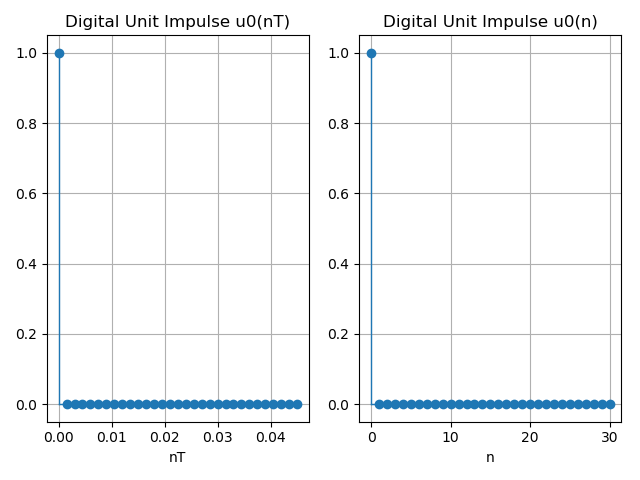
\includegraphics[width=0.7\textwidth]{img/signals/1.png}
    \caption{Цифровой единичный импульс}%
\end{figure}
\begin{equation}
    u_0 (nT) = \begin{cases}
        1, &n = 0;\\
        0, &n \ne 0.
    \end{cases}
\end{equation}

\clearpage
\subsection{Цифровой единичный скачок}
\begin{figure}[h]
    \centering
    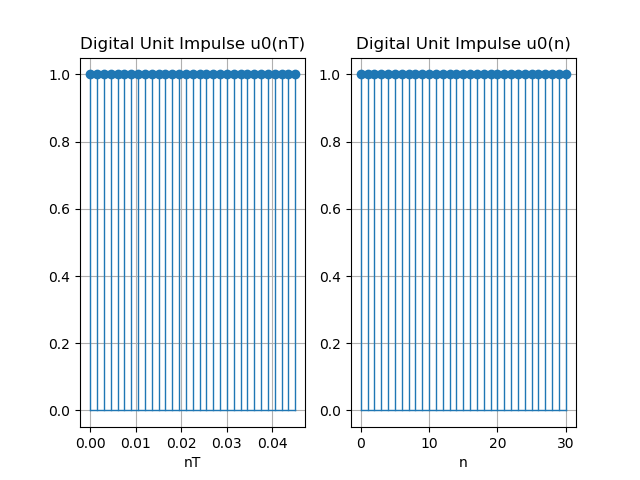
\includegraphics[width=0.7\textwidth]{img/signals/2.png}
    \caption{Цифровой единичный скачок}%
\end{figure}
\FloatBarrier{}
\textbf{Цифровой единичный скачок} --- результат дискретизации аналогового скачка.
\begin{equation}
    u_1 (nT) = \begin{cases}
        1, &n \ge 0;\\
        0, &n < 0.
    \end{cases}
\end{equation}

\clearpage
\subsection{Дискретная экспонента}
\begin{figure}[h]
    \centering
    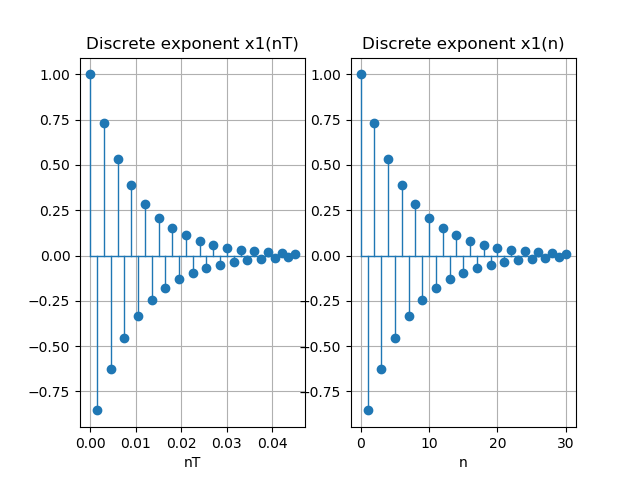
\includegraphics[width=0.7\textwidth]{img/signals/3.png}
    \caption{Дискретная экспонента}%
    \label{img:}
\end{figure}

\textbf{Дискретная экспонента} --- результат дискретизации аналоговой экспоненты.

\begin{equation}
    x_1(n) = \begin{cases}
        a^n, &n \ge 0 \\
        0, &n < 0,
    \end{cases}
\end{equation}
где $n$ --- дискретное нормированное время. От $a$ зависит, будет ли сменяться знак экспоненты.

\clearpage
\subsection{Дискретный гармонический сигнал}
\begin{equation}
    x_2(n) = C \cos (\hat{ \omega_0 } n),
\end{equation}
где $C$ --- амплитуда сигнала, $\hat{ \omega_0 }$ --- частота сигнала

\subsection{Дискретный комплексный гармонический сигнал}
\begin{figure}[h]
    \centering
    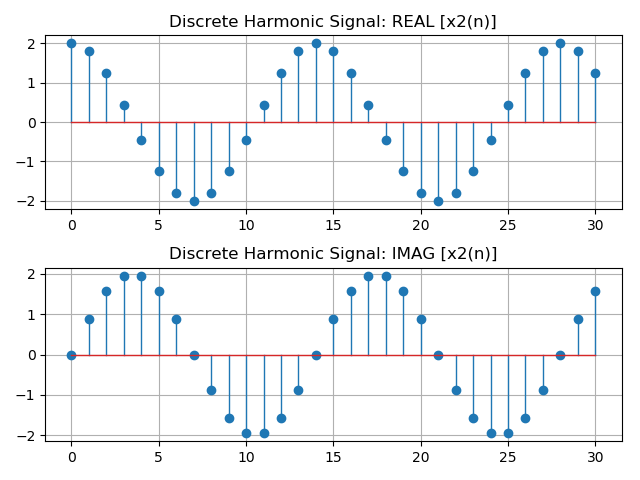
\includegraphics[width=0.7\textwidth]{img/signals/4.png}
    \caption{Графики вещественной и комплексной частей гармонического сигнала}%
\end{figure}

\begin{equation}
    x_2(n) = C e ^{j\hat{ \omega_0 } n}
\end{equation}

\clearpage
\subsection{Дискретный прямоугольный импульс}
\begin{figure}[h]
    \centering
    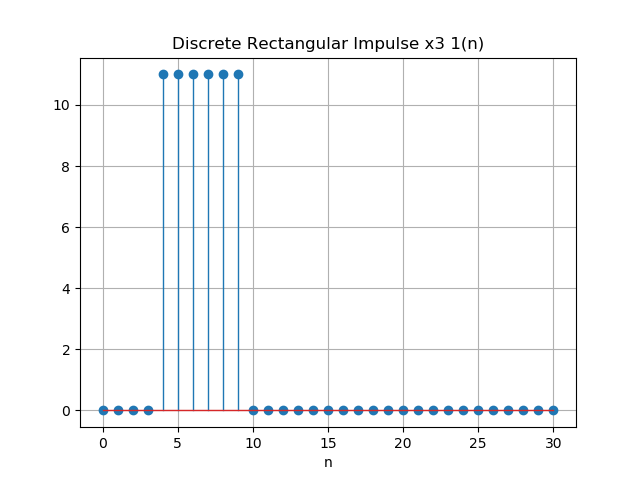
\includegraphics[width=0.7\textwidth]{img/signals/6.png}
    \caption{График дискретного прямоугольного импульса}%
\end{figure}
\begin{equation}
    x_3 (n) = \begin{cases}
        U, &n_0 \le n \le (n_0 + n_\text{imp} --- 1 );\\
        0, &\text{иначе},
    \end{cases}
\end{equation}
где $U$ --- амплитуда, $n_0$ --- момент начала, $n_\text{imp} $ --- длительность.

\clearpage
\subsection{Дискретный треугольный импульс}
\begin{figure}[h]
    \centering
    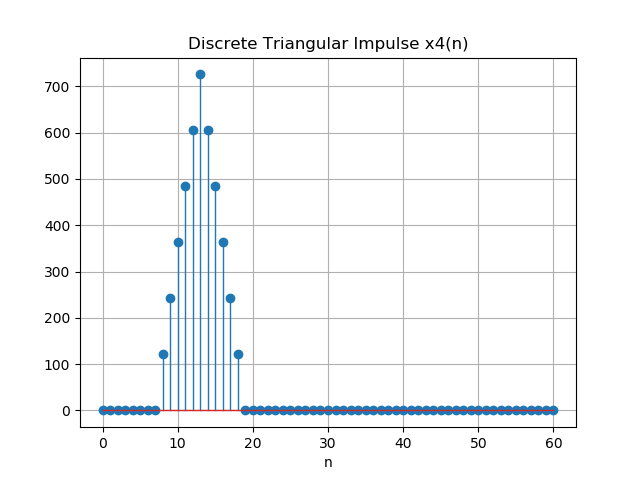
\includegraphics[width=0.7\textwidth]{img/signals/7.png}
    \caption{График дискретного треугольного импульса}
\end{figure}
Можно получить сверткой дискретного прямоугольного импульса самим с собой на интервале $L$.

Аналитическая запись свертки:
\begin{equation}
    x_4(t) = x_3(t) * x_3(t) = \sum\limits_{\tau = 0}^{N} x_3(\tau) x_3(t - \tau),
\end{equation}
где $x_3(\tau)$:
\begin{equation}
    x_3(\tau) = \begin{cases}
        U, & n_0 \le \tau \le (n_0 + n_{imp} - 1)\\
        0, & \text{иначе}
    \end{cases}
\end{equation}
Длина свертки: $L = 2N - 1$.


\section{Линейные дискретные системы. Описание во временной области}
\subsection{Линейные дискретные системы}\label{subsec:lds}
\textbf{Система обработки сигнала} --- объект, выполняющий требуемое преобразование входного сигнала \textbf{(воздействия)} в выходной \textbf{(реакцию)}.

\begin{figure}[h]
    \centering
    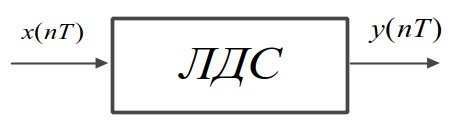
\includegraphics[width=0.6\textwidth]{img/S002.jpg}
    \caption{Схематичное изображение ЛДС}%
\end{figure}

Система --- \textbf{линейная}, если она отвечает условиям \textbf{аддитивности} и \textbf{однородности}.

\textbf{Аддитивность} --- реакция на сумму воздействий равна сумме реакций на воздействия:

\textbf{Однородность} --- воздействию, умноженному на весовой коэффициент, соответствует реакция, умноженная на тот коэффициент.

\begin{equation}
    L\{ a_1 x_1(n) \pm a_2 x_2(n) \pm \ldots \} = a_1 L\{ x_1(n)\} \pm a_2 L\{x_2(n)\} \pm \ldots,
\end{equation}
где: $x_i(n)$ --- воздействие, $a_i$ --- весовой коэффициент.

Система --- \textbf{дискретная}, если она преобразует дискретное воздействие в дискретную реакцию.

Система --- \textbf{стационарная}, если её реакция инвариантна по отношению к начала отсчёта времени. По умолчанию рассматриваем стационарные линейные дискретные системы (ЛДС).

\subsection{Описание ЛДС во временной области}
Основная характеристика во временной области --- \textbf{импульсная характеристика (ИХ)}, $h(n)$ --- реакция на цифровой единичный импульс $u_0(n)$ при ННУ.

\textbf{Соотношение вход/выход} ЛДС --- однозначно связано с ИХ, имеет вид линейной свертки:
\begin{equation}\label{eq:in_out}
    y(nT) = \sum^{\infty}_{m=0} h[ (n - m)T ] x(mT) = \sum^{\infty}_{m=0} h(mT) x [ (n-m)T ],
\end{equation}
\begin{equation}\label{eq:in_out:2}
    y(n) = \sum^{\infty}_{m=0} h(n-m)x(m) = \sum^{\infty}_{m=0} h(m) x(n-m).
\end{equation}

\textbf{Передаточная функция} --- однозначно связана с соотношением вход/выход, имеет вид \textbf{разностного уравнения (РУ)}:
\begin{equation}\label{eq:ru}
    y(n) = \underbrace{\sum^{N-1}_{i=0} b_i x(n-i)}_\text{Нерекурсивная часть} - \underbrace{\sum^{M-1}_{k=1} a_k y(n-k)}_\text{Рекурсивная часть},
\end{equation}
где:
\begin{itemize}
    \item $b_i, a_k$ --- вещественные константы (параметры ЛДС)
    \item $i, k$ --- задержки воздействия, реакции
    \item $(N-1), (M-1)$ --- константы (максимальные задержки)
    \item $x(n)$ --- воздействие
    \item $y(n)$ --- реакция
\end{itemize}

Вычисление реакции по формуле свертки или разностому уравнению осуществляется методов прямой подстановке при начальных нулевых условиях.

Типы ЛДС:
\begin{itemize}
    \item \textbf{Рекурсивные} --- реакция зависит от текущего и предшествующих отсчётов воздействия и предшествующих отсчётов реакции.

        $ \exists k: a_k \ne 0$.

        Имеют бесконечную ИХ \textbf{(БИХ-ЛДС)}.
    \item \textbf{Нерекурсивные} --- реакция зависит только от текущего и предшествующих отсчётов воздействия и не зависит от отсчётов реакции.

        $\forall k: a_k = 0$.

        Имеют конечную ИХ \textbf{(КИХ-ЛДС)}. ИХ КИХ-ЛДС совпадает с коэффициентами $b_i$: $h(n) = b_i, n=i$
\end{itemize}

\section{Линейные дискретные системы. Описание в $z$-области}
См.~\ref{subsec:lds} (\nameref{subsec:lds}).

Основная характеристика --- \textbf{передаточная функция} (ПФ) --- $z$-изображение импульской характеристики:
\begin{equation}\label{eq:tf}
    H(z) = \sum^{N-1}_{n=0} h(n) z^{-n} = \frac{Y(z)}{X(z)},
\end{equation}
где $Y(z)$ --- $z$-изображение реакции, $X(z)$ --- $z$-изображение воздействия.

Передаточная функция с использованим разностного уравнения:
\begin{equation}
    H(z) = \frac{ \sum^{N-1}_{i=0} b_i z^{-i} }{1 + \sum^{M-1}_{k=1} a_k z^{-k}},
\end{equation}
где:
\begin{itemize}
    \item $z^{-i}, z^{-k}$ --- задержки воздействия и реакции,
    \item $a_k$ --- коэффициенты передаточной функции.
\end{itemize}

Для нерекурсивных ЛДС:
\begin{equation}
    H(z) = \sum^{N-1}_{i=0} b_i z^{-i} = \sum^{N-1}_{n=0} h(n) z^{-n}.
\end{equation}

\textbf{Порядок рекурсивной ЛДС} равен порядку знаменателя передаточной функции $(M-1)$ при условии $(N-1) \le (M-1)$.

\textbf{Порядок нерекурсивной ДЛС} равен $(N-1)$.

\textbf{Нули ПФ} --- корни числителя, \textbf{Полюса (особые точки) ПФ} --- корни знамененателя. \textbf{Карта нулей и полюсов} --- $z$-плоскость с единичной окружностью, нулями и полюсами.

Нули и полюсы --- попарно комплексно сопряженные числа.

Для \textbf{устойчивой ЛДС} полюса расположены внутри единичной окружности.

ПФ рекурсивных ЛДС может быть представлена следующими разновидностями:
\begin{itemize}
    \item Произведение простейших множителей:
        \begin{equation}
            H(z) = b_0 \prod^{M-1}_{k=1} \frac{1 - z_{0^k}z^{-1}}{1-z_{*^k}z^{-1}},
        \end{equation}
        где:
        \begin{itemize}
            \item $z_{0^k}$ --- $k$-й нуль, $z_{*^k}$ --- $k$-й полюс.
        \end{itemize}
    \item Произведение множителей второго порядка:
        \begin{equation}
            H(z) = \prod^{L}_{k=1} \frac{b_{0k} + \tilde{b}_{1k} z^{-1} + \tilde{b}_{2k}z^{-2}}{1 + a_{1k} z^{-1} + a_{2k} z^{-2}},
        \end{equation}
        где:
        \begin{itemize}
            \item $b_{0k}, \tilde{b}_{1k}, \tilde{b}_{2k}, a_{1k}, a_{2k}$ --- вещественные коэффициенты рекурсивных звеньев 2-го порядка (биквадратов),
            \item $L$ --- количество звеньев:
                \begin{equation}
                L = int( \frac{M-1}{2} ).
                \end{equation}
        \end{itemize}
    \item Сумма простых дробей:
        \begin{equation}
            H(z) = \sum^{M-1}_{k=1} H_k(z) = \sum^{M-1}_{k=1} \frac{A_k}{1-z_{*^k}z^{-1}},
        \end{equation}
        где:
        \begin{itemize}
            \item $z_{*^k}$ --- простой (некратный) полюс,
            \item $A_k$ --- коэффициент разложения при полюсе.
        \end{itemize}
\end{itemize}

\section{Линейные дискретные системы. Описание в частотной области}
См.~\ref{subsec:lds} (\nameref{subsec:lds}).
Основная характеристика --- \textbf{комплексная частотная характеристика} --- Фурье-изображение ИХ:
\begin{equation}\label{eq:complex_freq}
    H(e^{j \hat{ \omega }}) = \sum^{\infty}_{n=0} h(n) e^{-j \hat{ \omega } n},
\end{equation}
где $\hat{ \omega }$ --- нормированная частота (рад):
\begin{equation}
    \hat{ \omega } = \omega T.
\end{equation}

Связь ЧХ и ПФ:
\begin{equation}
    H(e^{j \hat{ \omega }}) = H(z) \big\vert_{z=e^{j \hat{w}}} = \dfrac{ \sum\limits^{N-1}_{i=0} b_i e^{-ji \hat{ \omega }} }{1 + \sum\limits^{M-1}_{k=1} a_k e^{-jk \hat{ \omega }}},
\end{equation}
где:
\begin{itemize}
    \item $b_i$ --- параметры нерекурсивной части ЛДС,
    \item $a_i$ --- параметры рекурсивной части ЛДС.
\end{itemize}

В показательной форме:
\begin{equation}
    H(e^{j \hat{ \omega }}) = \left| H(e^{j \hat{ \omega }}) \right| e^{j \cdot \arg \{ H(e^{j \hat{ \omega }}) \} } = A(\hat{ \omega }) e^{j \varphi(\hat{ \omega })},
\end{equation}
где $A(\hat{ \omega })$ --- АЧХ, $\varphi( \hat{ \omega } )$ --- ФЧХ.

\textbf{Амлитудно-частотная характеристика (АЧХ)} --- частотная зависимость отношения амплитуды реакции к амплитуде гармонического воздействия в установившемся режиме.

\textbf{Фазочастнотная характеристика (ФЧХ)} --- частотная зависимость разности фаз реакции и гармонического воздействия в установившемся режиме.

Свойства АЧХ и ФЧХ:
\begin{itemize}
    \item АЧХ и ФЧХ --- периодические функции;
    \item АЧХ --- четная функция частоты, ФЧХ --- нечетная;
    \item АЧХ и ФЧХ рассчитываются в основной полосе частот для систем с вещественными параметрами;
    \item по карте нулей и полюсов можно определить местоположение минимумов, максимумов и нулей АЧХ в основной полосе частот;
    \item Частота комплексно сопряженного полюса соответствует частоте максимума АЧХ (приблизительно);
    \item Частота комплексно сопряженного нуля соответствует частоте минимума АЧХ (приблизительно), если радиус-вектор полюса меньше 1, и нуля АЧХ, если радиус-вектор равен 1. В точке нуля АЧХ наблюдается скачок на $\pi$;
    \item Вещественным нулям соответствует нуль АЧХ на границе основной полосы частот $0$ и/или $\pi$.
\end{itemize}

\section{Основные характеристики ЛДС. Соотношение вход / выход. Устойчивость ЛДС}
\begin{itemize}
    \item Во временной области --- импульсная характеристика, соотношение вход/выход (cм.~\ref{eq:in_out},~\ref{eq:in_out:2})
    \item В $z$-области --- передаточная функция (см.~\ref{eq:tf})
    \item В частнотной области --- комплексная частотная характеристика (см.~\ref{eq:complex_freq})
\end{itemize}

ЛДС называется \textbf{устойчивой}, если её реакция на любое ограниченное воздействие является ограниченной.

Критерии устойчивости:
\begin{itemize}
    \item Критерий во временной области
    \begin{itemize}
        \item ЛДС устойчива, если ряд отсчётов импульсной характеристики является абсолютно сходящимся
        \item КИХ-фильтры устойчивы по определению
        \item БИХ-фильтры требуют проверки на устойчивость
    \end{itemize}
    \item Критерий в $z$-области\\
        ЛДС устойчива, если все полюса располагаются внутри единичного круга. Граница круга соотвествует \textbf{границе устойчивости}.

        Чем дальше полюс от границы круга, тем больше \textbf{запас устойчивости}.

        В неустойчивой системе возможны \textbf{самовозбуждения}.
\end{itemize}

\section{$z$-преобразование и его свойства}\label{sec:loran}
\subsection{$z$-преобразование и преобразование Лапласа}
$z$-преобразования связано с \textbf{преобразованием Лапласа}:
\begin{equation}
    X(p) = \int_0^\infty x(t) e^{-pt} dt,
\end{equation}
где:
\begin{itemize}
    \item $x(t)$ --- непрерывная функция времени (оригинал),
    \item $X(p)$ --- изображение
    \item $p = \sigma + j \omega$ --- опреатор Лапласа.
\end{itemize}

Преобразование Лапласа справедливо в области абсолютной сходимости несобственного интеграла.

\textbf{Дискретное преобразование Лапласа}:
\begin{equation}
    t \to nT,
\end{equation}
\begin{equation}
    X(e^{pt}) = \sum^{\infty}_{n=0} x(nT) e^{-pnt}.
\end{equation}

\textbf{$z$-преобразование}:
\begin{equation}
    z = e^{pt},
\end{equation}
\begin{equation}
    X(z) = \sum^{\infty}_{i=1} x(nT) z^{-n},
\end{equation}
где:
\begin{itemize}
    \item $x(nT)$ --- функция дискретного времени,
    \item $X(z)$ --- $z$-изображение $x(nT)$.
\end{itemize}

$z$-преобразование справедливо в области абсолютной сходимости ряда
\begin{equation}
    \sum^{\infty}_{n=0} | x(nT) z^{-n} | < \infty.
\end{equation}

\subsection{Свойства $z$-преобразования}
\begin{enumerate}
    \item Линейность
        \begin{equation}
            \begin{split}
                x(n) &= a_1 x_1(n) + a_2 x_2(n) + \ldots\\
                X(z) &= a_1 X_1(z) + a_2 X_2(z) + \ldots
            \end{split}
        \end{equation}
    \item Теорема о задержке
        \begin{equation}
            \begin{split}
                x(n) \leftrightarrow X(z),\\
                x(n-m) \leftrightarrow X(z) z^{-m}.
            \end{split}
        \end{equation}
    \item Теорема о свертке
        \begin{equation}
            \begin{split}
                x(n) = \sum^{\infty}_{m=0} x_1(m) x_2(n-m) \leftrightarrow X(z) = X_1(z) X_2(z).
            \end{split}
        \end{equation}
\end{enumerate}

\section{Структуры ЛДС}
\textbf{Структура} отображает алгоритм определения реакции по РУ (см.~\ref{eq:ru}) и определяется видом передаточной функции.

Для рекурсивных звеньев 2-го поряд с передаточной функцией:
\begin{equation}
    H(z) = \frac{b_0 + b_1 z^{-1} + b_2 z^{-2}}{1 + a_1 z^{-1} + a_2 z^{-2}},
\end{equation}
где $b_0, b_1, b_2$ --- нерекурсивная часть, $a_1, a_2$ --- рекурсивная часть,
и разностным уравнением
\begin{equation}
    y(n) = b_0 x(n) + b_1 x(n-1) + b_2 x(n-2) - a_1 y(n-1) - a_2 y(n-2)
\end{equation}
поддерживаются далее перечисленные структуры.

\subsection{Прямая структура (Direct Form I)}
\begin{figure}[h]
    \centering
    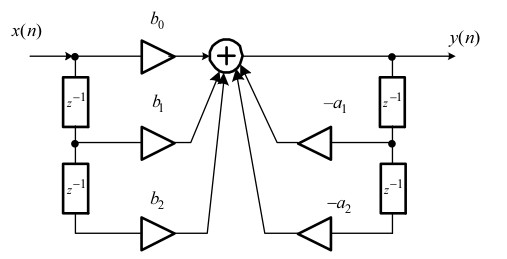
\includegraphics[width=0.85\textwidth]{img/S003.jpg}
    \caption{Прямая структура}%
    \label{img:df1}
\end{figure}
\clearpage

\subsection{Прямая транспонированная структура (Direct Form I Transposed)}
\begin{figure}[h]
    \centering
    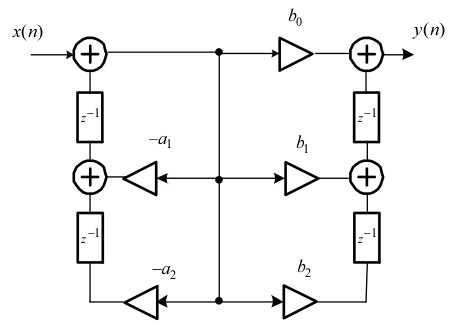
\includegraphics[width=0.75\textwidth]{img/S004.jpg}
    \caption{Прямая транспонированная структура}%
    \label{img:df1t}
\end{figure}

\subsection{Прямая каноническая структура (Direct Form II)}
\begin{figure}[h]
    \centering
    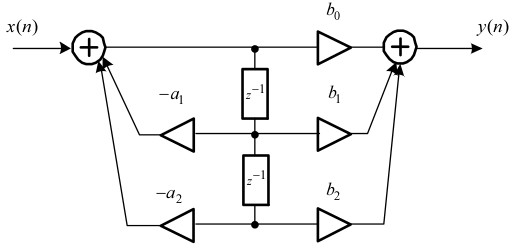
\includegraphics[width=0.8\textwidth]{img/S005.jpg}
    \caption{Прямая каноническая структура}%
    \label{img:df2}
\end{figure}
\clearpage

\subsection{Прямая каноническая транспонированная структура (Direct Form II Transposed)}
\begin{figure}[h]
    \centering
    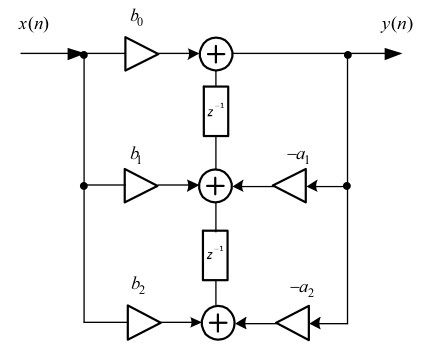
\includegraphics[width=0.7\textwidth]{img/S006.jpg}
    \caption{Прямая каноническая транспонированная структура}%
    \label{img:df2t}
\end{figure}
\FloatBarrier{}

\subsection{Каскадная (последовательная) структура}
Для звеньев с передаточной функцией:
\begin{equation}
    H(z) = \prod^K_{k=1} H_k (z),
\end{equation}
где $H_k(z)$:
\begin{equation}
    H_k(z) = \frac{b_{0k} + b_{1k} z^{-1} + b_{2k} z^{-2}}{1 + a_{1k} z^{-1} + a_{2k} z^{-2}}.
\end{equation}
\begin{figure}[h]
    \centering
    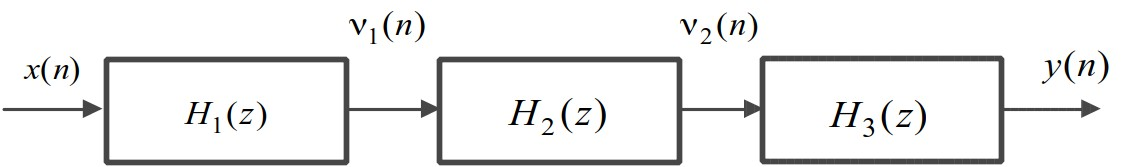
\includegraphics[width=\textwidth]{img/S007.jpg}
    \caption{Последовательная структура}%
    \label{img:cons}
\end{figure}

Система разностных уравнений:
\begin{equation}
    \begin{cases}
        \nu_1(n) &= b_{01} x(n) + b_{11} x(n-1) + b_{21} x(n-2) - a_{11} \nu_1(n-1) - a_{21} \nu_1(n-2);\\
        \nu_2(n) &= b_{02} \nu_1(n) + b_{12}\nu_1(n-1) + b_{22} \nu_1(n-2) - a_{12} \nu_2(n-1) - a_{22} \nu_2(n-2);\\
        y(n) &= b_{03} \nu_2(n) + b_{13} \nu_2(n-1) + b_{23} \nu_2 (n-2) - a_{13} y(n-1) - a_{23} y(n-2).
    \end{cases}
\end{equation}

\subsection{Параллельная структура}
Для звеньв с передаточной функцией
\begin{equation}
    H(z) = \sum^{K}_{k=} H_k(z),
\end{equation}
где $H_k(z)$:
\begin{equation}
    H_k(z) = \frac{B_{0k} + B_{1k}z^{-1}}{1+a_{1k}z^{-1}+a_{2k}z^{-2}}.
\end{equation}

\begin{figure}[h]
    \centering
    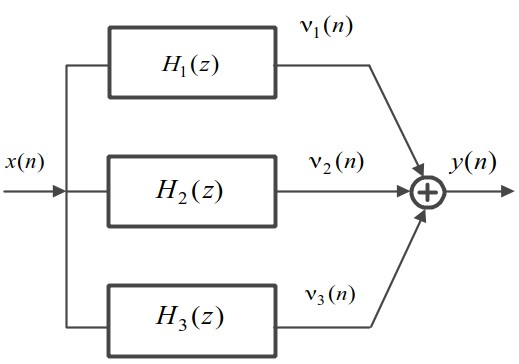
\includegraphics[width=0.7\textwidth]{img/S008.jpg}
    \caption{Параллельная структура}%
    \label{img:parr}
\end{figure}
\FloatBarrier{}

Для нерекурсивной (КИХ) ЛДС, передаточная функция:
\begin{equation}
    H(z) = \sum^{N-1}_{i=0} b_i z^{-i},
\end{equation}
разностное уравнение:
\begin{equation}
    y(n) = \sum^{N-1}_{i=0} b_i x(n-i).
\end{equation}
Для КИХ ЛДС 2-го порядка:
\begin{equation}
    y(n) = b_0 x(n) + b_1 x(n-1) + b_2 x(n-2).
\end{equation}

\begin{figure}[h]
    \centering
    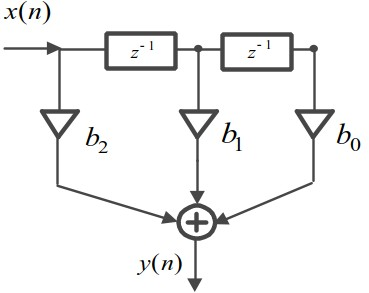
\includegraphics[width=0.7\textwidth]{img/S009.jpg}
    \caption{Параллеьная структура для КИХ ЛДС}%
    \label{img:cons:kix}
\end{figure}


\section{Цифровые фильтры}
\textbf{Цифровой фильтр (ЦФ)} --- ЛДС, выполняющая преобразование входной последовательности в выходную по алгоритму, описываемому разностным уравнением, структурой, реализованной аппаратно, программно или аппаратно-программно.

\subsection{Проектирование ЦФ}
\begin{enumerate}
    \item \textbf{Синтез ЦФ}
        \begin{enumerate}
            \item \textit{Выбор типа ЦФ}\\
                КИХ-фильтр (FIR) для КИХ ЛДС, БИХ-фильтр (IIR) для БИХ ЛДС.
            \item \textit{Задание требований к характеристикам ЦФ}\\
                Зависят от типа и назначения ЦФ.\\
                По умолчанию подразумевают частотно-избирательные ЦФ --- выполняющие селекцию спектральных составляющих. \\
                Для них типы избирательности:
                \begin{itemize}
                    \item ФНЧ (фильтр нижних частот);
                    \item ФВЧ (фильтр верхних частот);
                    \item ПФ (полосовой фильтр);
                    \item РФ (режекторный фильтр).
                \end{itemize}
            \item \textit{Выбор метода синтеза}
                Зависит от типа и дополнительных требований.
            \item \textit{Расчёт передаточной функции ЦФ}
            \item \textit{Выбор структуры ЦФ}
        \end{enumerate}
    \item \textbf{Моделирование структуры ЦФ с учетом эффекта квантования}
    \item \textbf{Реализация структуры ЦФ}\\
        Способы реализации:
        \begin{itemize}
            \item аппаратная (с использованием ПЛИС, ЦПОС);
            \item программная (MATLAB, SIMULINK);
            \item программно-аппаратная.
        \end{itemize}
\end{enumerate}

\section{Синтех КИХ-фильтров методом окон}
\subsection{КИХ-фильтр}\label{subsec:fir}
\textbf{КИХ-фильтр} описывается передаточной функцией:
\begin{equation}
    H(z) = \sum^{N-1}_{i=0} b_i z^{-i} = \sum^{N-1}_{n=0}.
\end{equation}

\textbf{Длина} КИХ-фильтра --- число коэффициентов $N$, \textbf{порядок} --- порядок $R$ передаточной функции, равный $R=N-1$.

Особенности КИХ-фильтров:
\begin{itemize}
    \item возможность обеспечить строго линейную ФЧХ (ЛФЧХ);
    \item устойчивость по определению.
\end{itemize}

Линейная ФЧХ (с точностью до скачков на $\pi$, где АХЧ равна нулю) обеспечивается, если для ИХ $h(n)$ выполняется одно из условий:
\begin{itemize}
    \item симметрии: $h(n) = h(N - 1 - n)$;
    \item антисимметрии: $h(n) = -h(N-1-n)$,
\end{itemize}
где ось симметрии/антисимметрии проходит через $n=R/2$.

% TODO требования к АЧХ?

\begin{table}[h]
\centering
\caption{Типы КИХ-фильтров}
\begin{tabularx}{\textwidth}{@{}lllXl@{}}
\toprule
\textbf{Тип} & \textbf{Порядок $R$} & \textbf{ИХ $h(n)$} & \textbf{ЛФЧХ} & \textbf{ЦФ}      \\ \midrule
1            & четный               & симметричная       & $\varphi(\hat{\omega}) = - \dfrac{\hat{\omega}R}{2} $ & ФНЧ, ФВЧ, ПФ, РФ \\
2            & нечетный             & симметричная       & $\varphi(\hat{\omega}) = - \dfrac{\hat{\omega}R}{2}$ & ФНЧ, ПФ          \\
2            & четный               & несимметричная     & $ \varphi(\hat{\omega}) = \dfrac{\pi}{2} - \dfrac{\hat{\omega}R}{2}$ & ПФ, ЦПГ          \\
3            & нечетный             & несимметричная     & $\varphi(\hat{\omega}) = \dfrac{\pi}{2} - \dfrac{\hat{\omega}R}{2}$ & ФВЧ, ПФ, ЦПГ, ЦД \\ \bottomrule
\end{tabularx}
\end{table}

\clearpage
\subsection{Структуры КИХ-фильтров с ЛФЧХ}
\begin{figure}[h]
    \centering
    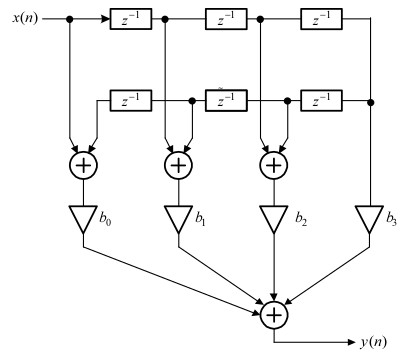
\includegraphics[width=0.52\textwidth]{img/S010.jpg}
    \caption{Прямая приведенненная с симметричной ИХ для КИх-фильтра 1-го типа}%
\end{figure}

\begin{figure}[h]
    \centering
    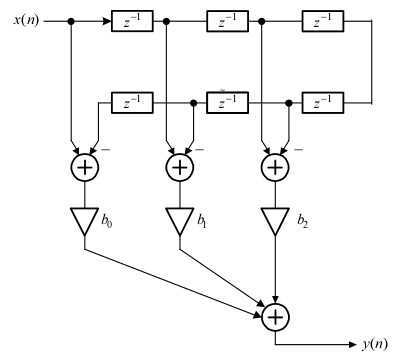
\includegraphics[width=0.53\textwidth]{img/S011.jpg}
    \caption{Прямая приведенная с антисимметричной ИХ для КИХ-фильтра 3-го типа}%
\end{figure}
\FloatBarrier{}

\subsection{Процедура синтеза КИХ-фильтров методом окон}
\begin{enumerate}
    \item Задание требований к АЧХ.
    \item Оценка порядка фильтра $R$ и выбор окна.\\
        \textbf{Окно} --- весовая функция $w(n)$ --- вещественная неотрицательная последовательность $N=R+1$, максимальная в центре и монотонно спадающая к границам.
    \item Расчёт ИХ идеального фильтра $h_\text{и}(n)$, выделенной окном Дирихле (прямоугольным).\\
        ИХ рассчитывается по известным аналическим формулам для типов фильтров. Обязательный параметр --- частота разрыва, на которой нормированая АЧХ равна $0.5$.
    \item Расчёт ИХ реального фильтра с симметричной $h(n)$ в виде произведения:
        \begin{equation}
            h(n) = h_\text{и}(n)w(n)
        \end{equation}
    \item Проверка выполнения требований к АЧХ.\\
        Заключается в проверки максимальных по модулю отклонений АЧХ от идеальной АЧХ.\\
        Производится поиск минимального порядка, при котором выполняются требования.
    \item Выбор структуры КИХ-фильтра.
\end{enumerate}

\section{Синтез КИХ-фильтров методом наилучшей равномерной (чебышевской) аппроксимации}
См.~\ref{subsec:fir} (КИХ-фильтр).

Метод чебышевской аппроксимации позволяет синтезировать \textbf{оптимальный КИХ-фильтр} --- фильтр наименьшего возможного порядка, удовлетворяющий заданным требованиям к АЧХ.

Коэффициенты оптимального КИХ-фильтра определяются поиском минимум функционала --- критерия Чебышева (наилучшего равномерного приближения).

\textbf{Расчёт весов}:
\begin{itemize}
    \item $1$ присваивается полосе с наибольшим максимально допустимым отклонением;
    \item в остальных полосах --- рассчитываются как отношение наибольшего максимально допустимого отклонения к максимально допустимому отклонению в данной полосе.
\end{itemize}

Согласно \textbf{теореме Чебышева}, минимум максимальной (по модулю) взвешенной ошибки аппроксимации $\delta_{\min\max}$ достигается в \textbf{точках альтернанса} --- частотах, на которых максимальное (по по модулю) взвешенное отклонение амплитудной функции от идеальной АЧХ минимально, одинаково и чередуется по знаку.

\begin{table}[h]
\centering
\caption{Количество точек альтернанса и порядок КИХ-фильтра}
\begin{tabular}{@{}lllll@{}}
\toprule
\textbf{Тип} & \textbf{Порядок $R$} & \textbf{ИХ $h(n)$} & \textbf{Число точек альтернанса} & \textbf{Порядок фильтра} \\ \midrule
1            & четный               & симметричная       & $m=\frac{R}{2} + 2$             & $R=2m-4$                 \\
2            & нечетный             & симметричная       & $m=\frac{R-1}{2} + 2$            & $R=2m-3$                 \\
2            & четный               & несимметричная     & $m=\frac{R}{2} + 1$             & $R=2m-2$                 \\
3            & нечетный             & несимметричная     & $m=\frac{R-1}{2} + 1$           & $R=2m-3$                 \\ \bottomrule
\end{tabular}
\end{table}

Синтез КИХ-фильтра сводится к расчёту его импульсной характеристики.

Шаги процедуры:
\begin{enumerate}
    \item Задание требований к АЧХ
    \item Оценка порядка фильтра $R$
    \item Расчёт ИХ фильтра.\\
        Производится с помощью численного метода --- \textbf{алгоритма Паркса---Мак-Клиллена}
    \item Проверка выполнения требований к АЧХ.\\
        Заключается в сравнении взвешенной ошибки аппроксимации $\delta_{\min\max}$ с допустимым взвешенным отклонением $\delta_{\max}$ АЧХ от идеальный АЧХ, равным:
        \begin{itemize}
            \item Для ФНЧ, ФВЧ:
                \begin{equation}
                    \delta_{\max} = \max\{\delta_1, \delta_2\}
                \end{equation}
            \item Для ПФ:
                \begin{equation}
                    \delta_{\max} = \max\{\delta_{21}, \delta_{1}, \delta_{22}\}
                \end{equation}
            \item Для РФ:
                \begin{equation}
                    \delta_{\max} = \max\{\delta_{11}, \delta_{2}, \delta_{12}\}
                \end{equation}
        \end{itemize}
        Производится итеративный поиск минимального порядка, при котором выполняются требования к АЧХ.
    \item Выбор структуры КИХ-фильтра
\end{enumerate}

\section{Синтез БИХ-фильтров}
\subsection{БИХ-фильтр}
\textbf{БИХ-фильтр} --- фильтр с бесконечной импульсной характеристикой.

Передаточная функция:
\begin{equation}
    H(z) = \frac{ \sum^{N-1}_{i=0} b_i z^{-i} }{1 + \sum^{M-1}_{k=1} a_k z^{-k}}
\end{equation}
и при $(N-1) \le (M-1)$ имеет порядок, равный $R = (M-1)$.

Особенности:
\begin{itemize}
    \item \textbf{нелинейность ФЧХ}, т.е. наличие фазовых искажений;
    \item необходимость проверки на устойчивость.
\end{itemize}

\subsection{Синтех методом билинейного $z$-преобразования}
Синтез заключается в расчёте передаточной функции. Метод билинейного $z$-преобразования основан на использовании аналогового фильтра-прототипа (АФП):
\begin{enumerate}
    \item Задание требований к характеристике затухания АЧХ БИХ-фильтра
    \item Формирование требования к АЧХ АФП\\
        Связь граничных частот АФП $\Omega$ с граничными частотами БИХ-фильтра:
        \begin{equation}
            \Omega = \frac{2}{t} \tan \frac{\omega T}{2},
        \end{equation}
        которая в шкале частот в герцах соответствует зависимости между частотами АФП $F$ и БИХ-фильтра $f$:
        \begin{equation}
            F = \frac{f_\text{д}}{\pi} \tan \frac{\pi f}{f_\text{д}},
        \end{equation}
    \item Выбор типа БИХ-фильтра.\\
    \begin{table}[h]
    \centering
    \caption{Типы БИХ-фильтров}
    \begin{tabular}{@{}lll@{}}
    \toprule
    \textbf{Название} & \textbf{АЧХ в ПП}   & \textbf{АЧХ в ПЗ} \\ \midrule
    Баттерворта       & максимально плоская & монотонная        \\
    Чебышева I рода   & равноволновая       & монотонная        \\
    Чебышева II рода  & максимально плоская & равноволновая     \\
    Золотарева-Кауэра & равноволновая       & равноволновая     \\ \bottomrule
    \end{tabular}
    \end{table}
    \item Расчёт передаточной функции $H_a(p)$
    \item Преобразование передаточной функции АФП $H_a(p)$ в передаточную функцию БИХ-фильтра на основе формулы билинейного $z$-преобразования:
        \begin{equation}
            p = \frac{2}{T} \cdot \frac{1 - z^{-1}}{1 + z^{-1}}.
        \end{equation}
    \item Выбор структуры БИХ-фильтра
\end{enumerate}

\section{Описание дискретных сигналов в $z$-области}
См.~\ref{sec:loran} (\nameref{sec:loran})

\subsection{Некоторые сигналы в $z$-области}
\begin{equation}
    u_0(n) = \begin{cases}
        1, &n=0\\
        0, &n\ne 0
    \end{cases}
\end{equation}
--- дискретный единичный импульс,
\begin{equation}
    u_1(n) = \begin{cases}
        1, &n \ge 0\\
        0, &n < 0
    \end{cases}
\end{equation}
--- дискретный единичный скачок (функция Хевисайда).
\begin{table}[h]
    \centering
    \caption{Некоторые $z$-преобразования}
    \begin{tabular}{@{}ll@{}}
        \toprule
        \textbf{Сигнал $x(n)$} & $z$-изображение \\ \midrule
        $u_0(n)$ & 1 \\[6pt]
        $u_0(n-n_0)$ & $ \dfrac{1}{z^{n_0}} $ \\[12pt]
        $u_1(n)$ & $ \dfrac{z}{z-1} $ \\[12pt]
        ${(\pm a)}^n u_1(n)$ & $ \dfrac{1}{1 \mp az^{-1}} $ \\[12pt]
        $\cos( \omega_0 n ) u_1(n)$ & $ \dfrac{1 - z^{-1} \cos( \omega_0 )}{1 ---  2z^{-1} \cos( \omega_0 ) + z^{-2}} $ \\ \bottomrule
    \end{tabular}
\end{table}

\section{Описание дискретных сигналов в частотной области}
Фурье-изображение дискретного сигнала
\begin{equation}
    X(e^{j \omega T}) = \sum^{\infty}_{n=0} x(nT)e^{-j \omega Tn},
\end{equation}
где $T$ --- период дискретизации, $X(e^{j \omega T})$ --- спектральная плостность дискретного сигнала $x(n)$.

Спектральная плоскость в шкале дискретного нормированного времени и нормированной частоты:
\begin{equation}
    X(e^{j\hat{ \omega }} = \sum^{\infty}_{n=0} x(n)e^{-j \hat{ \omega }n}).
\end{equation}
Связь $z$-изображения со спектральной плотностью:
\begin{equation}
    X(e^{j\omega T}) = X(Z) \big\vert_{z=e^{j\omega T}}
\end{equation}

Вещественная и мнимая части спектральной последовательности --- \textbf{вещественный и мнимый спектр последовательности}.

Модуль спектральной плотности --- \textbf{амплитудный спектр последовательности}

Аргумет спектральной плотности --- \textbf{фазовый спектр последовательности}

\subsection{Свойства спектральной плотности}
\begin{enumerate}
    \item Непрерывность
    \item Период равен частоте дискретизации
    \item Линейность:
        \begin{equation}
            \begin{split}
                x(n) &= a_1 x_1(n) + a_2 x_2(n) + \ldots\\
                X(e^{j\hat{ \omega  }}) &= a_1 X_1(e^{j \hat{ \omega }}) + a_2 X_2(e^{j \hat{ \omega }}) + \ldots
            \end{split}
        \end{equation}
    \item Модуль спектральной функции --- четная функция частоты; аргумент спектральной функции --- нечетная функция частоты
    \item Равенство Парсеваля
    \begin{equation}
        \sum^{\infty}_{n=0} |x(nT)|^2 = \frac{T}{2\pi} \int^{ \frac{\pi}{T} }_{ \frac{-\pi}{T} } \big| X(e^{j \omega T}) \big|^2 d\omega
    \end{equation}
    \item Сдвиг спектральной плотности в частотной области:
        \begin{equation}
            x(nT) \Leftrightarrow X(e^{j\omega T}),
        \end{equation}
        \begin{equation}
            x(nT)e^{j\omega_0 nT} \Leftrightarrow X(e^{j(\omega - \omega_0)T}) - \text{сдвиг вправо},
        \end{equation}
        \begin{equation}
            x(nT)e^{-j\omega_0 nT} \Leftrightarrow X(e^{j(\omega + \omega_0)T}) - \text{сдвиг влево}.
        \end{equation}
    \item Сдвиг дискретного сигнала во временной области
    \begin{equation}
            x(nT) \Leftrightarrow X(e^{j\omega T}),
    \end{equation}
    \begin{equation}
        x((n-m)T) \Leftrightarrow X(e^{j \omega T}) e^{-j \omega mT}.
    \end{equation}
\end{enumerate}

\section{Дискретное преобразование Фурье (ДПФ)}
Прямое ДПФ:
\begin{equation}
    X(k) = \sum^{N-1}_{n=0} x(n) W^{nk}_N, k = 0, 1, \ldots, N - 1,
\end{equation}

обратное ДПФ:
\begin{equation}
    x(n) = \frac{1}{N} \sum^{N-1}_{k=0} X(k) W_N^{-nk}, n = 0, 1, \ldots, N - 1,
\end{equation}
где:
\begin{itemize}
    \item $x(n)$ --- исходный сигнал, $N$-точечная последовательность;
    \item $X(k)$ --- результат вычисления, $N$-точечное ДПФ;
    \item $N$ --- длина последовательности;
    \item $n = nT/T$ --- дискретное нормированное время (номер отсчёта);
    \item $T$ --- период дискретизации;
    \item $k$ --- дискретная нормированная частота;
    \item $k = k\Delta\omega / \Delta\omega$; $\Delta\omega$ --- период дискретизации (разрешение) по частоте.
\end{itemize}
\begin{equation*}
    \Delta\omega = \frac{\omega_\text{д}}{N} = \frac{2\pi}{NT}
\end{equation*}
\begin{equation*}
    W^{nk}_N = e^{-j \frac{2\pi}{N}nk} \text{--- поворачивающий множитель},
\end{equation*}
\begin{equation*}
    X(k) W^{-nk}_N = X(k) e^{j \frac{2\pi}{N} nk} \text{--- $k$-я дискретная гармоника,}
\end{equation*}
\begin{equation*}
    f = k \frac{f_\text{д}}{N} \text{--- значения абсолютных частот дискретных гармоник}.
\end{equation*}

\subsection{ДПФ периодической последовательности}
ДПФ $X(k)$ представляет собой её \textbf{спектр} с точностью до постоянного множителя $ \frac{I}{N}$.

Модуль ДПФ --- \textbf{амлитудный спектр} периодической последовательности, четная функция частоты. Для вещественной последовательности --- амплитудный спектр с точностью до постоянного множителя:
\begin{equation}
    \begin{cases}
        \frac{1}{N}, &k=0;\\
        \frac{2}{N}, &k\ne 0.
    \end{cases}
\end{equation}

Аргумент ДПФ --- \textbf{фазовый спектр}, нечетная функция частоты.

\subsection{Эффект растекания спектра}
Если хотя бы для одной из дискретных гармоник
\begin{equation}
    P_i = \frac{NT}{T_i} = \frac{Nf_i}{f_\text{д}} 
\end{equation}
оказывается нецелым числом, наблюдается \textbf{растекание спектра} --- появление в спектральном составе дополнительных составляющих. 

Эффект принципиально неустраним, но:
\begin{itemize}
    \item во многих случаях им можно пренебречь;
    \item можно использовать оконные функции.
\end{itemize}

\section{Методы непараметрического спектрального анализа}
\lipsum[1] %TODO

\section{Методы параметрического спектрального анализа}
\lipsum[1] %TODO

\section{Адаптивные фильтры и их применения}
\lipsum[1] %TODO


\end{document}
